
\chapter{Reconstruction of bone locations in 3D space}
The first project this report discusses is the reconstruction of 3D coordinates based on two stereoscopic, rectified images for the project ``XFish''. These images represent X-ray images of fish. They have been taken as incremental scans while a fish passes through the scanner over a conveyor belt. The X-ray emitter is considered to be a single point source and the X-ray detectors are two line detectors. 

As no access to such a physical scanner was available, a simulator had been written during a previous project. The simulator had the ability to generate X-ray images from 3D meshes. The objective of this project is to evaluate the maximum obtainable quality from the reconstruction of bones from the aforementioned X-Ray images. 

\section{Augmentations to the simulator}
The first step of the process was to find a means to perform perfect pixel matching on the two stereoscopic images. The best means to do this was to augment the simulator to produce additional images for each mesh. Each triangle of the mesh was labelled with a single colour and projected onto an image. This made it trivial to perform perfect matching as pixels can be compared by colour directly. Figure \ref{fig:labelled} shows two such images side by side. 

\begin{figure}
	\centering
	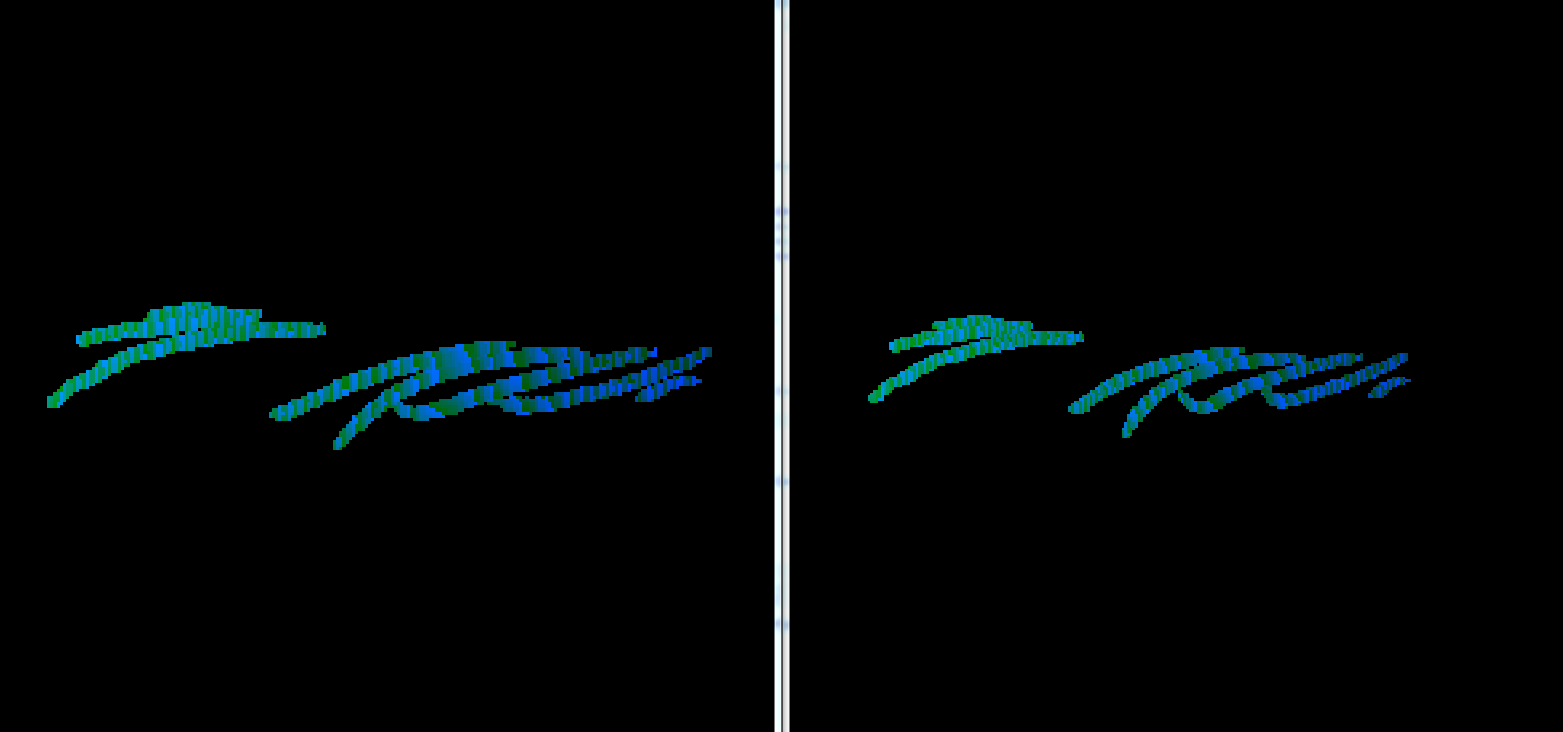
\includegraphics[width=160mm]{images/fish/test.png}
	\caption{A pair of labelled bones.}
	\label{fig:labelled}
\end{figure}

\section{The unprojection}
After pair of pixels on the images have been matched using the described method, it is unprojected using a number of known configuration values about the setup using several equations that have been derived for this purpose.

\subsection{Relevant variables}
Table \ref{table:imageProcessingVariables} lists a number of variables that are relevant for calculating the coordinates of a piece of bone inside the scanned fish. Note that component coordinates will in this chapter be referred to by a subscript letter. For example, the x-coordinate of point P is denoted by $P_x$.

\begin{table}[hpt!]
\begin{tabular}{ |p{2cm}|p{1.1cm}|p{12cm}| } 
 \hline
	\textbf{Variable} & \textbf{Type} & \textbf{Description} \\ 
\hline
	$D_1$, $D_2$ & Scalar & X coordinate of each of the detectors. \\ 
	\hline
	$D_{min}, D_{max}$ & Scalar & Y coordinates of the start and end of the active detector area, respectively. \\
	\hline
	D & Point & A single point to denote the origin point of both detectors, used whenever both values apply. \\
	\hline
	P & Point & Location of some piece of bone relative to the origin of the bounding box of the fish. The program aims to reconstruct this point. \\
	\hline
	E & Point & Location of the emitter.\\
	\hline
	F & Point & Origin of the bounding box of the fish being scanned. In the simulation this was considered to be at [0, 0, 0] at all times.\\
	\hline
	I & Point & Point that is only defined when P intersects an emitter-detector plane. Its Z coordinate is always 0 and its X coordinate is equal to $F_x$. Represents the location of the projected pixel on to the X-Ray image.\\
	\hline
	h & Scalar & Distance in the positive z direction that represents the distance between the detector and the bottom of the bounding box of the fish. This distance is mainly caused by the conveyor belt.\\
	\hline
	i & Point & Coordinate on X-Ray image. This point is deduced from the location of I. \\
	\hline
	R & Scalar & Units of distance represented by a single pixel. The X and Y axis are considered to have the same resolution. \\
\hline
\end{tabular}
\caption{Listing of relevant variables}
\label{table:imageProcessingVariables}
\end{table}

\subsection{Deduction of the original coordinate}

The following equation was deduced to unproject the x-coordinate:

\begin{equation}
P_x = \frac{I_{1x} (E_x - D_2) - I_{2x} (E_x - D_1)} {D_1 - D_2}
\end{equation}

\begin{equation}
P_y = \frac{E_y - I_y + D_x}{E_z}(P_z + F_z) + I_y + D_x - F_y
\end{equation}

\begin{equation}
P_z = \frac{E_z}{E_x - D_x}(I_x + P_x) - F_z 
\end{equation}

Note that the calculations of the individual components of the coordinate have to be done in the following order: $P_{x}$, $P_{z}$, $P_{y}$. 

\section{Results}
First, a verification of the simulator was done. The simulator casts a number of rays from the emitter on to both detectors. It then intersects these rays with the input mesh(es). These intersection points were then visualised together with the original mesh to verify their correctness. The result is shown in figure \ref{fig:simulator_points}.

\begin{figure}
	\centering
	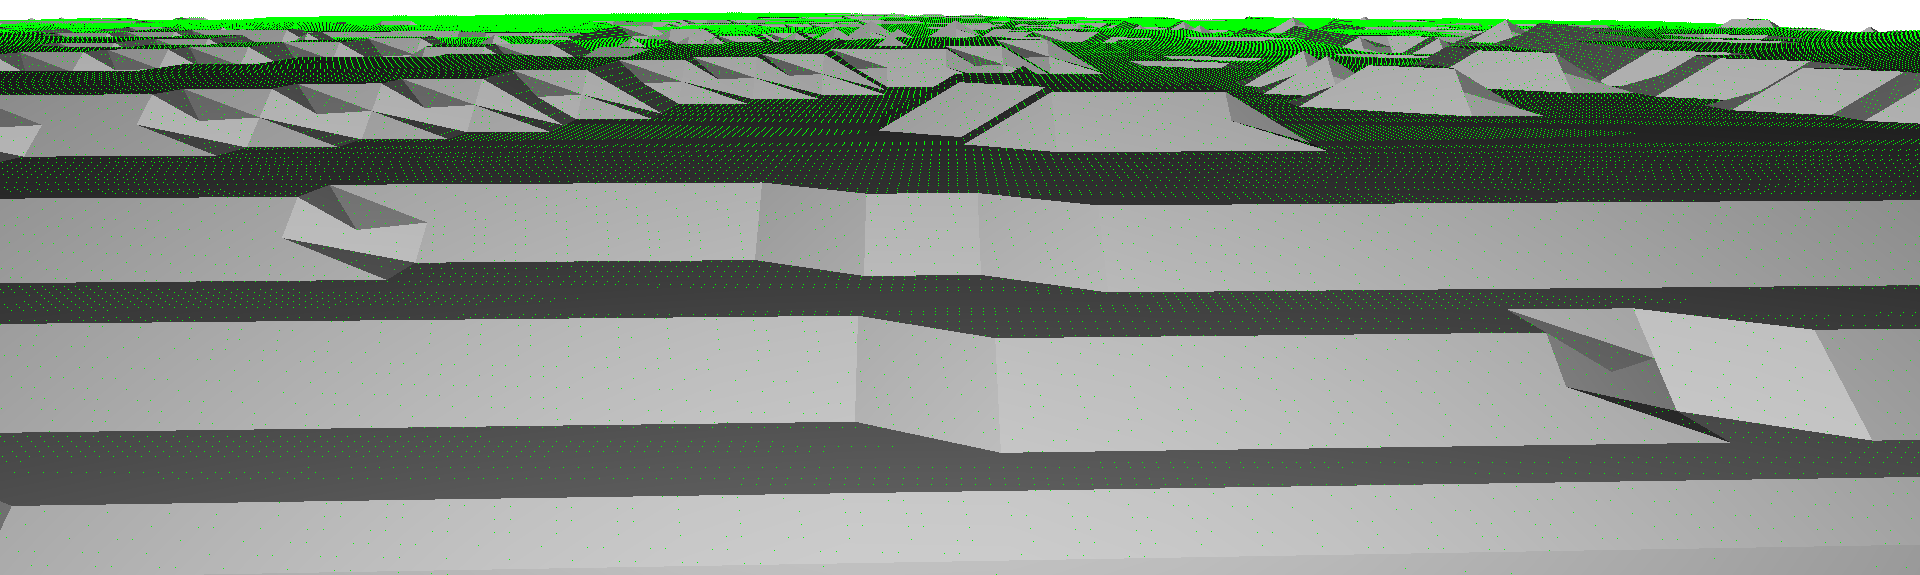
\includegraphics[width=160mm]{images/fish/rayIntersections.png}
	\caption{Visualised simulator ray intersection points. The gray surfaces belong to the 3D scanned mesh, the green points show ray intersections.}
	\label{fig:simulator_points}
\end{figure}

Next, the results of the bone reconstruction are shown in figure \ref{fig:bones_top}, \ref{fig:bones_front} and \ref{fig:bones_left}. The red dots represent the reconstructed points based on the coordinates from the stereoscopic images, and calculated with the equations listed before.

\begin{figure}
	\centering
	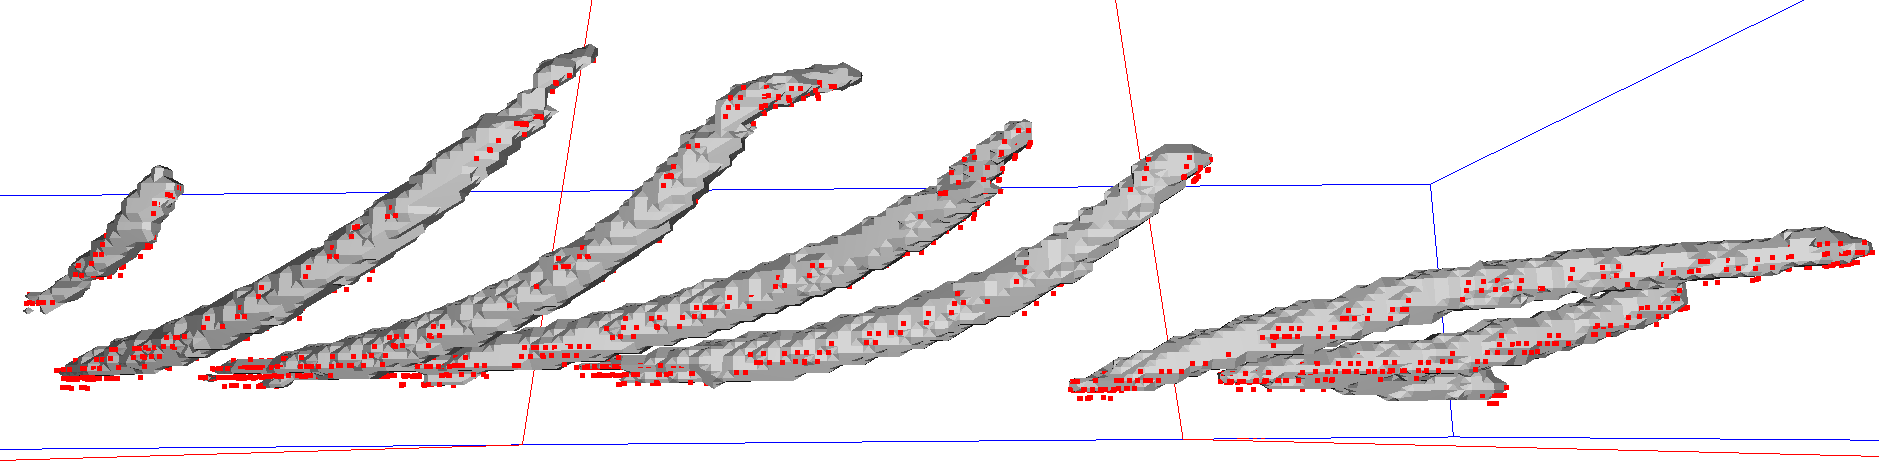
\includegraphics[width=160mm]{images/fish/bones1.png}
	\caption{Reconstructed points, seen from the top.}
	\label{fig:bones_top}
\end{figure}

\begin{figure}
	\centering
	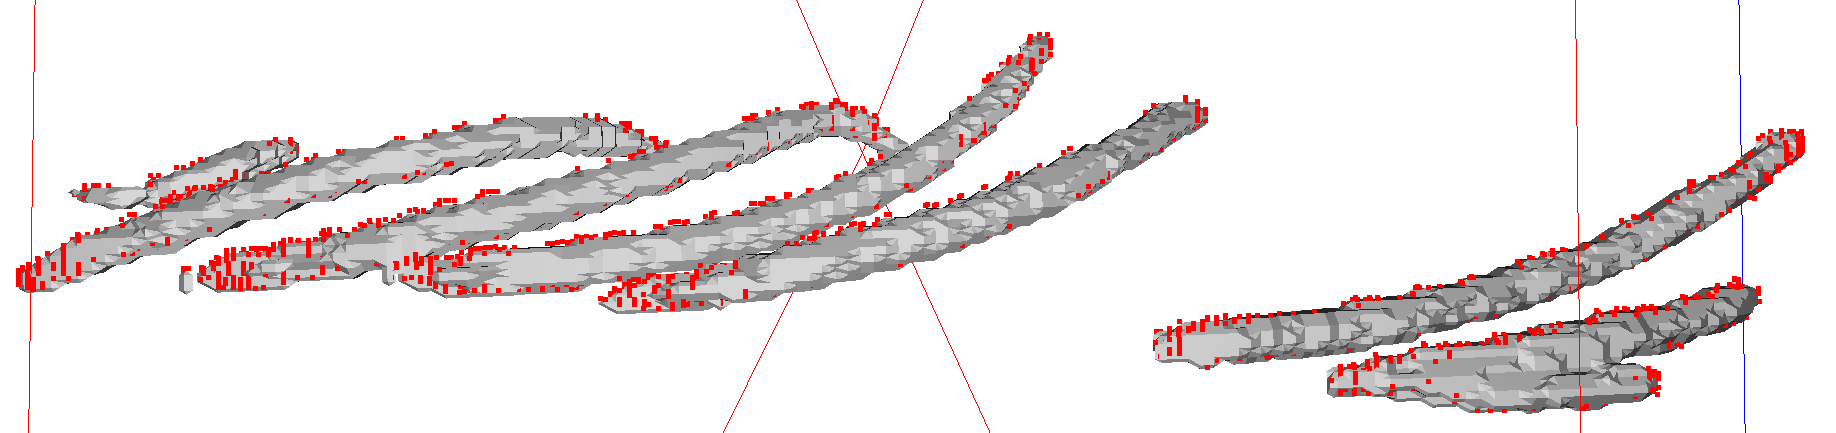
\includegraphics[width=160mm]{images/fish/bones2.png}
	\caption{Reconstructed bones, seen from the front.}
	\label{fig:bones_front}
\end{figure}

\begin{figure}
	\centering
	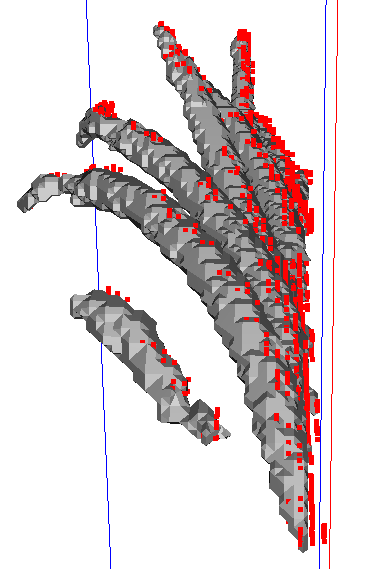
\includegraphics[width=50mm]{images/fish/bones3.png}
	\caption{Reconstructed bones, seen from the left.}
	\label{fig:bones_left}
\end{figure}

\section{Conclusion}
Most of the time spent on this project went into verifying the correctness of the existing code and the additional components written for this project specifically. Even so it appears there is still room for improvement of the quality of the unprojected coordinates. Still, the results that have been obtained thus far show much promise. 

Visual inspections show values close to the original position of the bone intersections, where most of the points end up inside the bones. For the purpose of cutting fish, it should be possible to obtain very good results iff a good coordinate pair matching algorithm is found and implemented.